\section{The software}
Now comes the software part.
In our mind, we wouldn't want to spend much time on programming.
We desired a plug-and-play solution, or something similar.
A software with easily controlling and possibly which can talk via ASCOM drivers with Stellarium (or others), PHD2 and others astrophotography programs.

\subsection{OnStep}
On the internet, we have found a great, open-source, free and customizable software called OnStep.\footnote{Wiki groups:\url{https://onstep.groups.io/g/main/wiki/3860}.\\Github:\url{https://github.com/hjd1964/OnStep}.}
We have followed the instructions for the WeMos D1 \(+\) CNC V3 project, configured the Config.h file and upload the sketch on the ESP32 board.
% \begin{minipage}
%     {0.5\textwidth}
%     \centering
%     \begin{tabular}{cc}
%         Variable & value \\
%         \hline
%         \texttt{PINMAP} & CNC3\\
%         \texttt{SERIAL\_A\_BAUD\_DEFAULT} & 115200 \\
%         \texttt{SERIAL\_B\_BAUD\_DEFAULT} & 115200 \\
%         \texttt{SERIAL\_C\_BAUD\_DEFAULT} &  ON \\
%         \texttt{MOUNT\_TYPE} & FORK \\
%         \texttt{BUZZER} & ON\\
%         \texttt{BUZZER\_STATE\_DEFAULT} & ON\\
%         \texttt{SLEW\_RATE\_BASE\_DESIRED} & 1.0\\
%         \texttt{TIME\_LOCATION\_SOURCE} & DS3231 \\
%         \texttt{PPS\_SENSE} & ON \\
%         \texttt{AXIS1\_STEPS\_PER\_DEGREE} & 38293.333 \\
%         \texttt{AXIS1\_STEPS\_PER\_WORMROT} & 38400\\ 
%         \texttt{AXIS1\_DRIVER\_MODEL} & DRV8825\\
%         \texttt{AXIS1\_DRIVER\_MICROSTEPS} & 32 \\
%         \texttt{AXIS1\_HOME\_DEFAULT} & 0\\
%         \texttt{AXIS2\_STEPS\_PER\_DEGREE} & 1002.66667 \\
%         \texttt{AXIS2\_DRIVER\_MODEL} & DRV8825 \\
%         \texttt{AXIS2\_DRIVER\_MICROSTEPS} & 32 \\
%         \texttt{AXIS2\_LIMIT\_MIN} & -35 \\
%         \texttt{AXIS2\_LIMIT\_MAX} & 80 \\
%         \texttt{AXIS2\_HOME\_DEFAULT} & 0\\
%         \texttt{TRACK\_AUTOSTART} & OFF \\
%         \texttt{BUZZER} & ON \\
%         \texttt{BUZZER\_STATE\_DEFAULT} & ON\\
%     \end{tabular}
%     \captionof{table}{Config.h variables we have changed.}
%     \label{fig:config_h}
% \end{minipage}

Finally, the box is placed on the mount and connected with the Ethernet cables to the motors

\subsection{PHD2}
\textit{Push It Dummy-2} is the software that controller the auto-guiding system.
PHD2 is telescope guiding software that simplifies the process of tracking a guide star, letting you concentrate on other aspects of deep-sky imaging.
There are plenty tutorials on the internet showing how to use PHD2, so we do not enter so much into details.\footnote{\url{https://www.youtube.com/watch?v=Kd4qzW7uV38} or the pdf \url{https://openphdguiding.org/man-dev/Basic_use.htm}.}
But we only want to stress out that, after few important configuration passes, the auto-guiding is really simple and promises very good results!

\subsubsection{Wizard configuration}
Connection is really simple using the "wizard" option suggested in every tutorials.
The "unbinned pixel size" is one of the first parameters you have to fix in the wizard which are not quite clear.
You should be able to get the unbinned pixel size from the camera spec sheet or the manufacturer's web site.
If this is not the case, you can get the unbinned pixel size by taking the dimension of the sensor and diving it by the number of pixels.

The "bin level" is the technique to combine proximal bins to form a "superpixel".\footnote{\url{https://www.photometrics.com/learn/imaging-topics/binning-2.}}
This has the effect of reducing the noise but at the price of reducing the image definition.

Another remarkable option to fill is the telescope mount's driver, which in this case are the ASCOM OnStep telescope drivers.

\begin{figure*}[t]
    \centering
    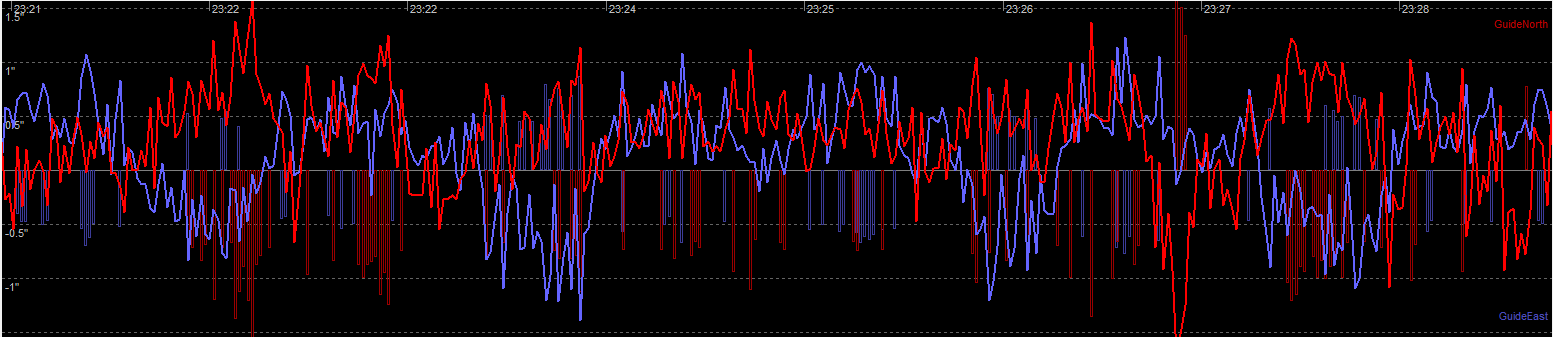
\includegraphics[scale=0.45]{analysis/PHD2/2021-12-09/guide-11-arcsec.png}
    \caption{DEC V3 test: PHD2 log view using arcseconds as units.}
    \label{fig:guide-11-arcsec}
\end{figure*}
\begin{figure*}[t]
    \centering
    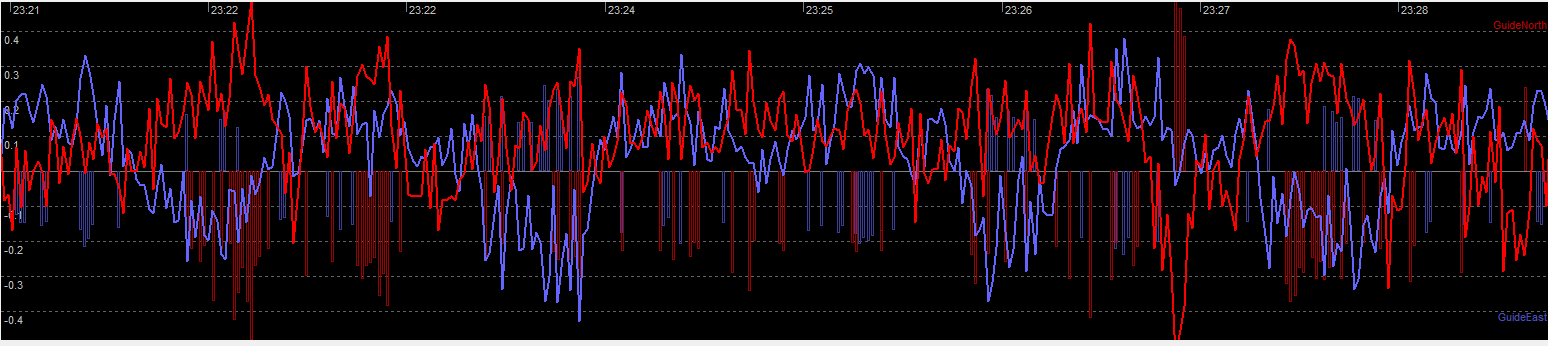
\includegraphics[scale=0.45]{analysis/PHD2/2021-12-09/guide-11-pixel.png}
    \caption{DEC V3 test: PHD2 log view using pixel as units.}
    \label{fig:guide-11-pixel}
\end{figure*}

\subsubsection{Dark libraries}
Before starting the first guiding session, it is useful to spend 5 minutes to create a dark library.
To do so, just press the "Dark" tool on the top and create a new dark library.
Cover the guidescope, and start the acquisition.

After the acquisition, remove the cover;
this should make clearer acquisitions.

\subsubsection{Connect all!}
After the configuration, press the first icon in the bottom left and press "connect all".
Now the camera and the mount are connected to PHD2.

\subsubsection{Calibration}
Search a bright star whose declination is between 10 to -10 degrees.
Start the acquisition pressing the "cycle" icon (the second from the left), then press the "star with a magnifying glass" that selects the most bright star.
Finally, push the PHD2 icon; this will start the calibration and requires few minutes.

\subsubsection{Guiding}
If dark libraries and calibration are done, the guiding can start.
If it is not present, search in the settings the plot visualization that let you know the adjustments that PHD2 is doing.
In our case, it is a useful tool to see if our work were precisely enough.        

A useful tool is the "use multiple stars" in the guiding settings.
The latter permits holding multiple star, and we think this is another improvement to stability in auto-guiding.


\subsection{Stellarium}
Stellarium is the software we use to search objects.
The impressive feature is that, after paring it via ASCOM drivers with the mount, it is possible to tell the telescope to move at the star pointed out in Stellarium.\footnote{See \url{https://www.youtube.com/watch?v=DUdYv311HFw}.}

The telescope is now free to start few tests to check the goodness of our work!